\documentclass[12pt]{article}
\usepackage[margin=1in]{geometry}
\usepackage{amsfonts, amsmath, amssymb}
\usepackage{polynom}
\usepackage{hyperref}
\usepackage{mathtools}
\hypersetup{
    colorlinks=true,
    linkcolor=blue,
    filecolor=magenta,      
    urlcolor=cyan,
}
\usepackage{graphicx}

\usepackage{fancyhdr}
\setlength{\headheight}{15pt}

\pagestyle{fancy}
\fancyhf{}

\rhead{
  Shengdong Li
  Calc 3
}

\rfoot{
  Page \thepage
}

\usepackage{indentfirst}

\begin{document}
\title{Response to Ankur Moolky}
\author{by Shengdong Li}
\date{2 October 2020}
\maketitle

\section{Intro}

Hello Ankur!

Great job with the initial post, it was easy to follow and well explained. I actually did my initial post on population too, except for me I did it on the entire US instead of just Oregon.

Below I'll solve for the general solution, draw a slope field, and make some observations.

\section{Solving for the General Solution}
I noticed that in your initial post, you already solved for the general solution, but as the prompt requires it I'll just show my work below...

$$
  \frac{dP}{dt}=0.0197P
$$
\begin{align}
  \intertext{First bring each variable to their own side}
  \frac{dP}{P}             & =0.0197dt             \\
  \intertext{Next we can integrate both sides}
  \int_{ }^{ }\frac{dP}{P} & =\int_{ }^{ }0.0197dt \\
  \\ln\left(P\right)&=0.0197t+C\\
  \intertext{Raise $e$ to the power of both sides}
  P                        & =e^{0.0197t+C}        \\
  \intertext{Finally, since $e^C$ is a constant we can take it out and set it as one $C$}
  \Aboxed{P                & =Ce^{0.0197t}}        \\
\end{align}
We got the same answer, so again, great job with the initial!
\section{All about the Slope Field}
\begin{figure}[h]
  \begin{center}
    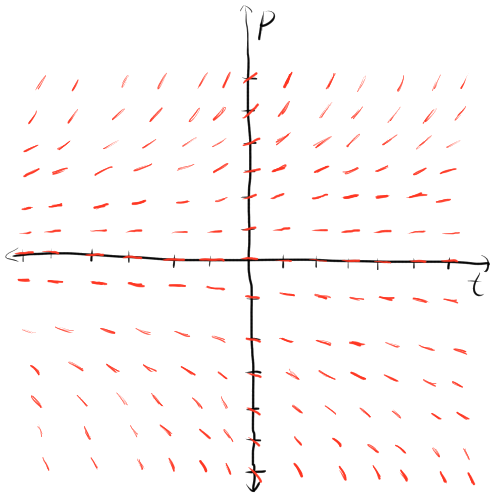
\includegraphics[scale=2]{disc-3-ankur-res-slope-field.png}
    \caption{\textit{Picture of slope field I drew for $\frac{dP}{dt}=0.0197P$.} Please also refer to much more clear \href{https://www.desmos.com/calculator/8abrp6yuwb}{\textcolor{blue}{desmos version}}, or see embed below}
  \end{center}
\end{figure}
\subsection{Observations}

As we can see, the differential does have an unstable equilibrium solution at $P=0$.

Another thing that I noticed about the slope field is that every slope for a given $P$  is the same. This suggests that $t$ does not actually affect the differential at any point, which makes sense because the rate of change of the population was assumed to be constant at the beginning of the problem. However, it might not be the most realistic, as in real life the change in population does change.

\end{document}